%%%%%%%%%%%%%%%%%%%%%%%%%%%%%%%%%%%%%%%%%%%%%%%%%%%%%%%%%%%%%%%%%%%%%%%%%%%%
%% Trim Size : 11in x 8.5in
%% Text Area : 9.6in (include Runningheads) x 7in
%% ws-ijbc.tex, 24 Jan 2010
%% Tex file to use with ws-ijbc.cls written in Latex2E.
%% The content, structure, format and layout of this style file is the
%% property of World Scientific Publishing Co. Pte. Ltd.
%%%%%%%%%%%%%%%%%%%%%%%%%%%%%%%%%%%%%%%%%%%%%%%%%%%%%%%%%%%%%%%%%%%%%%%%%%%%
%%

%\documentclass[draft]{ws-ijbc}
\documentclass{ws-ijbc}
\usepackage{ws-rotating}     % used only when sideways tables/figures are used
\usepackage{graphicx}
\usepackage{epstopdf}
\usepackage{mathrsfs}
\bibliographystyle{ws-ijbc}

\begin{document}

\catchline{}{}{}{}{} % Publisher's Area please ignore

\markboth{Author's Name}{Paper Title}

\title{A HETEROCLINIC CONNECTION BETWEEN TWO SADDLE SLOW MANIFOLDS IN THE OLSEN MODEL}

\author{Elle Musoke, Bernd Krauskopf and Hinke M. Osinga}

\address{Department of Mathematics, University of Auckland, Private Bag 92019\\
Auckland, 1142, New Zealand\\
elle.musoke@auckland.ac.nz}

\maketitle

\begin{history}
\received{(to be inserted by publisher)}
\end{history}

\begin{abstract}
The abstract should summarize the context, content and conclusions
of the paper. It should not contain any references or displayed
equations. Typeset the abstract in 10~pt Times Roman with
baselineskip of 12 pt, making an indentation of 1.6~cm on the left
and right margins.
\end{abstract}

\keywords{A list of 3--5 keywords are to be supplied.}
\section{Introduction}

Slow-fast dynamical systems are characterized by a separation of variables into those that evolve on a fast time scale and those that evolve on a slower time scale.  The separation of variables into fast and slow can be found in many systems in the world around us: chemical systems, neurons, electric circuits, lasers and predator-prey dynamics have been, among others, described by slow-fast models  \cite{BZ_reaction, Neurons,Circuits, lasers, Predator-Prey}.  By reason of their ubiquity, the various phenomena that arise from the multiple-time-scale nature of slow-fast systems are of significant interest. These have been be described for two- and three-dimensional systems by well-established theory \cite{canard_explosion, lents-rapides, enlacement,singular_hopf, folded_node,three}.  Small-amplitude limit cycles transitioning to larger-amplitude relaxation oscillations were studied in two dimensions, for example, the Van der Pol oscillator and Fitz-Hugh-Nagumo model \cite{canard_explosion, fitz-hugh-nagumo}.  In three-dimensional systems, periodic orbits with epochs of localized small-amplitude oscillations (SAOs) and epochs of large-amplitude oscillations (LAOs) have been observed \cite{BZ}.  The mechanisms that cause SAOs of these appropriately named mixed-mode oscillations (MMOs) are described in \cite{MMO}.  We now investigate novel phenomena that arise in four-dimensional slow-fast systems which may provide insight into undiscovered mechanisms for MMOs.


We consider a prototypical four-dimensional slow-fast dynamical system which exhibits MMOs.  We study the so-called Olsen model for peroxidase-oxidase reaction, first introduced by Lars F. Olsen in 1983  \cite{Olsen}, in a parameter regime corresponding to three fast and one slow variable.  Mechanisms for MMOs in the Olsen model were previously investigated in \cite{QSSA} after an assumption was made to reduce the model to a three-dimensional system.  Manifolds on which the flow progresses on the slower timescale were computed along with the manifolds consisting of trajectories that converged to them in forward and backwards time respectively.  These were found to be very insightful into the formation of MMOs as well as the cause of their particular geometry.  However, because of the assumptions used to reduce the model to a three-dimensional system, some of the computed manifolds were found to be of lower dimension than the corresponding manifolds in the full system.  In this research, we develop techniques for computing the same manifolds in the full four-dimensional model in the interest of studying their geometry and interactions with each other.  In particular, we focus on interactions between higher-dimensional manifolds that do not exist in systems of three dimensions or lower.


To better observe the separation between fast and slow variables, we use a change of coordinates described in \cite{Rescaling} and given by the system of ODEs
    
\begin{equation}
\begin{aligned}
\begin{cases}
\frac{dA}{dt} &= \mu - \alpha A - ABY, \\
\frac{dB}{dt} &= \varepsilon(1-BX - ABY), \\
\frac{dX}{dt} &= \frac{1}{\eta}(BX - X^2 +3ABY - \zeta X + \delta), \\
\frac{dY}{dt} &= \frac{\kappa}{\eta}(X^2 - Y - ABY),
\end{cases}
\end{aligned}
\label{equation_1}
\end{equation}
    
\noindent
where $(A, B, X, Y)\in\mathbb{R}^{4}$ are positive concentrations of chemicals.  The system parameters given by Greek letters in Table 1 are functions of original system parameters given in \cite{Olsen}. They were chosen to be the same as in \cite{Rescaling} with a minor modification.  Note that for notational convenience, we have substituted  $\varepsilon_{b}$ and $\varepsilon^{2}$ \cite{Rescaling} with $\varepsilon$ and $\eta$ respectively.

\begin{table}[h]
\tbl{System parameters for system (1)}
{\begin{tabular}{c  c  c  c  c  c  c  c  c} \\[-2pt]
\toprule
$\alpha$ & $\delta$ & $\varepsilon$ & $\eta$ & $\kappa$ & $\mu$ & $\zeta$ \\[6pt]
\hline\\[-2pt]
0.0912 & 1.2121e-04 & 0.0037 & 0.0540 & 3.7963 & 0.9697 & 0.9847\\[1pt]
\botrule
\end{tabular}}
\end{table}

The classification of variables as either slow or fast is not straightforward for the Olsen model because the variables are not consistently slow or fast over all regions of phase space.  In fact system (\ref{equation_1}) nominally has three different time scales.  The time-scaling parameters $\varepsilon$ and $\eta$ depend on the original system parameter $k_1$.  As suggested by \cite{Rescaling}, we decrease $k_{1}$ past $0.16$ to $0.1$ so that there are only two time scales.  We study a parameter regime corresponding to three fast variables, $A, X$ and $Y$, and one slow variable, $B$.

%Background section
\section{Background}
    
In the limit as $\varepsilon \rightarrow 0$, system (\ref{equation_1}) becomes
    
\begin{equation}
\begin{aligned}
\begin{cases}
\frac{dA}{dt} &= \mu - \alpha A - ABY, \\
\frac{dX}{dt} &= \frac{1}{\eta}(BX - X^2 +3ABY - \zeta X + \delta), \\
\frac{dY}{dt} &= \frac{\kappa}{\eta}(X^2 - Y - ABY),
\end{cases}
\end{aligned}
\label{equation_2}
\end{equation}
    
\noindent
in which $B$ is a parameter.  We refer to the three-dimensional system (\ref{equation_2}) as the layer equation or the fast subsystem.  If one first performs a time rescaling, $\tau = \varepsilon t$, and then considers the limit as $\varepsilon \rightarrow 0$ the system reduces to
    
 \begin{equation}
\begin{aligned}
\begin{cases}
0 &= \mu - \alpha A - ABY, \\
\frac{dB}{d\tau} &= (1-BX - ABY), \\
0 &= \frac{1}{\eta}(BX - X^2 +3ABY - \zeta X + \delta), \\
0 &= \frac{\kappa}{\eta}(X^2 - Y - ABY),
\end{cases}
\end{aligned}
\label{equation_3}
\end{equation}
    
\noindent
which is a differential algebraic system called the slow subsystem or the reduced system. The three algebraic equations in system (\ref{equation_3}) define a one-dimensional manifold called the critical manifold, $C$.  The flow in (\ref{equation_3}) is defined by the single differential equation for $B$ and it is confined to $C$.  

The critical manifold consists of equilibria of the fast subsystem for different values of $B$. These can be linearized about and their stability determined by the $3\times3$ Jacobian matrix of (\ref{equation_2}).  Equilibria at which the Jacobian's eigenvalues all have non-zero real parts are called hyperbolic, otherwise we say that the equilibrium is non-hyperbolic.  Non-hyperbolic equilibria lying on the critical manifold correspond to local bifurcations in (\ref{equation_2}).  The critical manifold has 11 branches near a stable MMO of interest, separated from each other by non-hyperbolic equilibria of the fast subsystem.

\begin{figure}[h]
\begin{center}
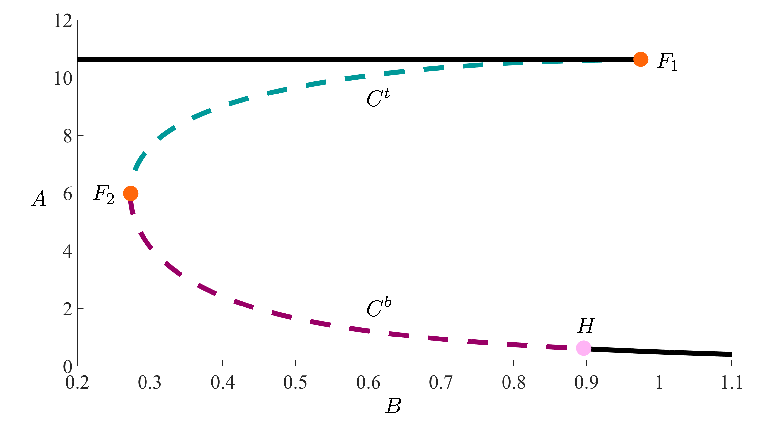
\includegraphics[page=1]{figures.pdf}
\end{center}
\caption{Physically relevant branches of the critical manifold of system (\ref{equation_1}) shown in projection onto the ($B$,$A$)-plane.  The branches labeled $C^t$ and $C^b$ and colored teal correspond to saddle equilibria of (\ref{equation_2}), solid curves indicate stable nodes.  The two saddle-node bifurcations are represented as orange dots and labeled $F_1$ and $F_2$ respectively.  The Hopf bifurcation is represented with a light pink dot and is labeled $H$.}
\label{critical_figure}
\end{figure}

Figure \ref{critical_figure} shows four branches of $C$ on which all variables are positive projected into the ($B$,$A$)-plane.  Seven nearby branches of $C$ are not shown, because they lie in regions where at least one of $A$, $B$, $X$, or $Y$ is negative and not physically relevant.  Of the branches shown in Figure \ref{critical_figure}, the topmost black branch consists of stable equilibria of (\ref{equation_2}) and is separated from the teal colored branch of saddle equilibria, denoted $C^t$, by a fold, shown in orange and denoted $F_1$, occurring at $B \approx 0.956$.  Equilibria $p \in C^t$ each have a two-dimensional linear stable space $E^s(p)$ and a one-dimensional linear unstable space $E^u(p)$.  The flow is from left to right near $C^t$ in the $(B,A)$-projection shown.  The fold $F_1$ has the appearance of a cusp in the ($B$,$A$)-projection, however ($B$,$X$)- and ($B$,$Y$)- projections show that this is truly a fold with respect to $B$.  Another fold, also shown in orange, separates $C^t$ from a lower raspberry colored branch of saddle equilibria and occurs at $B \approx 0.273$ and is denoted $F_2$.  The raspberry branch of saddle equilibria is denoted $C^b$ and is separated from a branch of stable equilibria on the right by a Hopf bifurcation, represented as a pink dot and denoted $H$, occurring at $B \approx 0.896$.  Equilibria on $C^b$ have each one stable and two unstable eigenvectors.  The flow is from right to left near $C^b$.
    
We denote the local stable and unstable manifolds of points $p \in C$ by $W^{s}_{loc}(p)$ and $W^{u}_{loc}(p)$.  These are the trajectories in \ref{equation_2} that converge to $p$ in forwards and backwards time respectively.  The saddle branch $C^t$ has a three-dimensional local stable manifold $W^{s}_{loc}(C^t)$ and a two-dimensional local unstable manifold $W^{u}_{loc}(C^t)$ defined as
    
$$W^{s}_{loc}(C^t) = \bigcup_{p \in C^t} W^{s}_{loc}(p), \hspace{1cm} W^{u}_{loc}(C^t) = \bigcup_{p \in C^t} W^{u}_{loc}(p).$$
    
\noindent
Similarly $C^b$ has a three-dimensional local unstable manifold and a two-dimensional local stable manifold defined as
    
$$W^{s}_{loc}(C^b) = \bigcup_{p \in C^b} W^{s}_{loc}(p), \hspace{1cm} W^{u}_{loc}(C^b) = \bigcup_{p \in C^b} W^{u}_{loc}(p).$$
    
We are interested in interactions between stable and unstable manifolds of $C^t$ and $C^b$ as $\varepsilon > 0$.  Although the branches $C^t$ and $C^b$ of the critical manifold are no longer invariant for $\varepsilon > 0$, Fenichel Theory guarantees that both $C^t$ and $C^b$ persist as locally-invariant manifolds called slow manifolds, denoted $S^t_\varepsilon$ and $S^b_\varepsilon$, that are not unique \cite{Fenichel}. Orbit segments that lie on a slow manifold remain slow for an $O(1)$ amount of slow timescale time.  Locally invariant means that solutions can only enter or leave the manifold via its edges.  
    
We can select a unique representative $S^t_\varepsilon$ by considering the slow manifold that remains slow for the longest amount of time.  The slow manifold $S^t_\varepsilon$ has the same dimension as $C^t$ and, as $\varepsilon \rightarrow 0$, orbit segments converge to $C^t$.  Since equilibria of (\ref{equation_2}) lying on $C^t$ are of saddle type, $C^t$ and $S^t_\epsilon$ are also of saddle type.  The slow manifold, $S^b_\varepsilon$, associated with $C^b$ can be similarly defined.
    
Fenichel Theory also guarantees that $W^{s}_{loc}(C^t)$ and $W^{u}_{loc}(C^t)$ persist as locally-invariant local stable and unstable manifolds of $S^t$ \cite{Fenichel}.  We define the stable manifold of $S^t_\varepsilon$ as a family of orbit segments, $W^s(S^t_\varepsilon)$, that have a fast approach to $S^t_\varepsilon$ and then stay close to it for an $O(1)$ amount of time.  Similarly, we define the unstable manifold as a family of orbit segments, $W^s(S^t_\varepsilon)$, that approach $S^t_\varepsilon$ in backward time and then stay close to it for an $O(1)$ amount of backward time.  According to Fenichel Theory, $W^s(S^t_\varepsilon)$ and $W^u(S^t_\varepsilon)$ have the same dimensions as $W^{s}_{loc}(C^t)$ and $W^{u}_{loc}(C^t)$ and lie at an $O(\varepsilon)$ distance away from them, respectively.  The manifolds $W^s(S^t_\varepsilon)$ and $W^u(S^t_\varepsilon)$ are not unique, however they can be made unique by imposing additional conditions.   We can similarly define the stable and unstable manifolds associated with $C^b$, denoted $W^s(S^b_\varepsilon)$ and $W^u(S^b_\varepsilon)$, respectively.
 
 %Saddle slow manifold section   
 
 \section{Computation of 1D saddle slow manifolds}
    
For the computation of a one-dimensional saddle slow manifold, we follow the presentation in \cite{Saeed_Paper} of a one-dimensional saddle slow manifold for a three-dimensional system.  Here we consider only the slow manifold $S^t_\varepsilon$ associated with $C^t$; the slow manifold $S^b_\varepsilon$ can be found in a similar manner.
    
The precise definition of the slow manifold $S^t_\varepsilon$ is given with respect to a closed interval $[B^t_{\mathrm{in}},B^t_{\mathrm{out}}]$ for the slow variable $B$.  The values for $B^t_{\mathrm{in}}$ and $B^t_{\mathrm{out}}$ are chosen such that the interval is contained in the interval defined by the $B$-coordinates of the two fold points $F_1$ and $F_2$.  Note that there is a segment in $C^t$ for which each point $p \in C^t$ is uniquely associated via its $B$-coordinaate with a value for $B_p \in [B^t_{\mathrm{in}},B^t_{\mathrm{out}}]$.  For each $B_p \in [B^t_{\mathrm{in}},B^t_{\mathrm{out}}]$ there is a unique point $p=(p_A,p_B,p_X,p_Y) \in C^t$ such that $p_B = B_p$.  We define a solid three-sphere $D_\delta(B_p)$ in the three-dimensional subsection $B=p_B$ that has radius $\delta$ and center $p$, given formally by

\begin{equation*}
D_\delta(B_p)=\{w \in \mathbb{R}^4 | w_B = B, |w-p| \leq \delta\}.
\end{equation*}
    
\noindent
The union $\mathscr{D} = \cup_{B \in [B^t_{\mathrm{in}}, B^t_{\mathrm{out}}]} D_\delta(B)$ forms a four-dimensional compact cylinder.  The radius $\delta$ is small, but it needs to be at least of $O(\varepsilon)$ to ensure that $S^t_\varepsilon$ lies in $\mathscr{D}$.  The one-parameter family of orbit segments that enter $\mathscr{D}$ via $D_\delta(B^t_{\mathrm{in}})$ and exit via $D_\delta(B^t_{\mathrm{out}})$ are candidates for $S^t_\varepsilon$.   We impose the additional condition that $S^t_\varepsilon$ must have maximal integration time in $\mathscr{D}$ to select a unique candidate to represent $S^t_\varepsilon$.  This condition may be interpreted as selecting $S^t_\varepsilon$ such that it enters $\mathscr{D}$ via $W^{s}(S^t_\varepsilon)$ and exits via $W^{u}(S^t_\varepsilon)$.
    
The set-up is similar to the set-up described in \cite{Saeed_Paper} with the difference that $D_\delta(B^t_{\mathrm{in}})$ and $D_\delta(B^t_{\mathrm{out}})$ are three-spheres rather than two-dimensional disks and $\mathscr{D}$ is four dimensional rather than three dimensional.  Plotted in green in Figure \ref{tube_figure} is a projection of the unique representative of $S^t_\varepsilon$.  Sketched in purple is $\mathscr{D}$ with the spheres $D_\delta(B^t_{\mathrm{in}})$ and $D_\delta(B^t_{\mathrm{out}})$ at either end.

\begin{figure}[h]
\begin{center}
\includegraphics[page=2]{figures.pdf}
\end{center}
\caption{A visualization of the slow manifold definition projected into the $(B,A)$-plane.  The spheres $D_\delta(B^t_{\mathrm{in}})$ and $D_\delta(B^t_{\mathrm{out}})$ are represented by purple disks at either end of a four-dimensional cylinder, also represented in purple.  A computation of the slow manifold is plotted in green and labelled $S^t_\varepsilon$.}
\label{tube_figure}
\end{figure}

\subsection{Boundary Value Set-Up}
    
We compute $S^t_\varepsilon$ by setting up an appropriately defined two-point boundary-value problem (2PBVP) with the pseudo-arclength continuation package \textsc{Auto} \cite{AUTO}.  We view $S^t_\varepsilon$ as an orbit segment $\mathbf{u} = \{\mathbf{u}(s)| 0 \leq s \leq 1 \}$ of the rescaled system


\begin{equation}
\frac{d\mathbf{u}}{ds} = TF(\mathbf{u}),
\label{equation_4}
\end{equation}
    
\noindent
where $\mathbf{u}(s) = (A(s), B(s), X(s), Y(s)) \in \mathbb{R}^4$ is the vector of chemical concentrations, $F$ is the right-hand side of (\ref{equation_1}) and $T$ is the total integration time on the fast timescale, $t=Ts$.
    
To obtain an initial solution of (\ref{equation_4}), we perform a homotopy step as follows.  First, we choose $B^t_{\mathrm{out}} = 0.75$ at a value that corresponds to a point $p^t_{\mathrm{out}} \in C^t$ close to $F_1$.  We then impose the conditions
    
\begin{equation}
\mathbf{u}(0) \in E^u(C^t),
\label{BC3}
\end{equation}
and
\begin{equation}
\mathbf{u}(1) \in E^s(p^t_{\mathrm{out}}),
\label{BC2}
\end{equation}
\noindent
that each impose two conditions on $\mathbf{u}(0)$ and $\mathbf{u}(1)$, respectively.  The point $p$ is then a solution to the two-point boundary-value problem defined by (\ref{equation_4})--(\ref{BC2}) with $T=0$.  We then  decrease $\mathbf{u}_B(0)$ towards $S1$ while the total integration time increases.  The integration is stopped when $\mathbf{u}_B(0)=0.4$, corresponding to the point $p^* \in C^t$, before it reaches $F_2$.
    
We remark that $D_\delta(B^t_{\mathrm{in}})$ defines a three-parameter family of orbit segments with initial conditions in the sphere.  We can refine our search for orbits that enter the cylinder via $D_\delta(B^t_{\mathrm{in}})$ and exit it via $D_\delta(B^t_{\mathrm{out}})$ by observing that, because $S^t_\varepsilon$ is of saddle type, the initial point of a candidate orbit segment must lie in a small neighborhood of $W^s(S^t_\varepsilon)$ in the sphere $D_\delta(B^t_{\mathrm{in}})$.  Similarly the end point must remain in a small neighborhood of $W^u(S^t_\varepsilon)$ in the sphere $D_\delta(B^t_{\mathrm{out}})$.
    
We define the two-dimensional plane $\Phi = \{E^u(p^t_{\mathrm{in}}) + \begin{bmatrix} 0 & 0 & 0 & Y \end{bmatrix}^{T}| Y \in \mathbb{R} \}$ that is transverse to $W^s(S^t_\varepsilon) \cap D_{\delta}(B^t_{\mathrm{in}})$ and contains $E^u(p^*)$.  We impose the boundary conditions
    
\begin{equation}
\mathbf{u}(0) \in \Phi
\label{BC1}
\end{equation}
    
\noindent
which also imposes two conditions on $\mathbf{u}(0)$.  The orbit segment resulting from the homotopy step is then a solution to the 2PBVP defined by (\ref{equation_4}), \ref{BC2}, and (\ref{BC1}).  The total integration time $T$ is a free parameter in this 2PBVP, which means that there exists a one-parameter family of solutions.  To select a unique orbit segment from this solution family, we impose the additional condition that $T$ be locally maximal.  This will be the orbit segment which locally has the longest slow segment in the geometric sense and will be the best approximation of $S^t_\varepsilon$.  In the case where there are two such candidates, we choose one.
    
In the final continuation run we increase the integration time until a fold in $T$ is detected.  The resulting orbit segment approximates the saddle slow manifold, $S^t_\varepsilon$.
   
A projection of $S^t_\varepsilon$ into the $(B,A)$-plane is shown as the green curve in Figure \ref{tube_figure}.  A keen observer will note that, near $D_\delta(B^t_{\mathrm{in}})$, $S^t_\varepsilon$ includes a segment of sharp decrease mostly in the $A$-direction.  This is due to the final step in our computation, where we restrict $\mathbf{u}(0)$ to move in the plane $\Sigma$.  In order to increase the integration time, $\mathbf{u}(0)$ then moves toward the intersection of $W^s(S^t_\varepsilon)$ with $\Sigma$ while $\mathbf{u}(1)$ moves toward the intersection of $E^s(p^t_{\mathrm{out}})$ with $W^u(S^t_\varepsilon)$.  The fold in $T$ signals when $u(0)$ and $u(1)$ are near respective intersection points and the result is an orbit segment containing fast segments lying on $W^s(S^t_\varepsilon)$ and $W^u(S^t_\varepsilon)$.  In Figure \ref{tube_figure}, the segment lying on $W^u(S^t_\varepsilon)$ is so short that it is not visible.  We obtain an approximation of $S^t_\varepsilon$ that does not include fast segments by restricting the orbit segment further within the interval $[B^t_{\mathrm{in}},B^t_{\mathrm{out}}]$.
   
An approximation of the slow manifold associated with $C^b$ can be computed in the same way by choosing $B^b_{\mathrm{in}}$ near $H$, and $B^b_{\mathrm{out}}$ near $S2$ in the above definition.  We choose $B^b_{\mathrm{in}}=B^b_{\mathrm{out}}$ smaller than and near $H_B$.
        

%\begin{multicols}{2}
\section{The Main Text}
\noindent Contributions are to be in English. Authors are
encouraged to have their contribution checked for grammar.
American spelling should be used. Abbreviations are allowed but
should be spelt out in full when first used. Integers ten and
below are to be spelt out. Italicize foreign language phrases
(e.g.~Latin, French).

The text is to be typeset in 11~pt Times \hbox{Roman},
single-spaced with baselineskip of 13~pt. Text area is 17.8~cm (7
inches) across and 24.4~cm (9.6 inches) deep (including running
title). Final pagination and insertion of running titles will be
done by the publisher.

\section{Major Headings}
Major headings should be typeset in boldface, with the first
letter of important words capitalized.

\subsection{Subheadings}
Subheadings should be typeset in bold italics, with the first
letter of first word capitalized and the section number in
boldface.

\subsubsection{Sub-subheadings}
Typeset in italics (section number to be in roman) and capitalize
the first letter of the first word only.

\subsection{Numbering and spacing}
Sections, subsections and sub-subsections are numbered with Arabic
numerals. Use double spacing after major and subheadings, and
single spacing after sub-subheadings.

\section{Lists of Items}
Lists are broadly classified into four major categories that can
randomly be used as desired by the author:
\begin{alphlist}[(d)]
\item Numbered list.
\item Lettered list.
\item Unnumbered list.
\item Bulleted list.
\end{alphlist}

\subsection{Numbered and lettered list}

\begin{arabiclist}[(5)]
\item The \verb|\begin{arabiclist}[]| command is used for the arabic
number list (arabic numbers appearing within parenthesis), e.g.,
(1), (2), etc.

\smallskip

\item The \verb|\begin{romanlist}[]| command is used for the roman
number list (roman numbers appearing within parenthesis), e.g., (i),
(ii), etc.

\smallskip

\item The \verb|\begin{Romanlist}[]| command is used for the cap roman
\hbox{number list} (cap roman numbers appearing within parenthesis),
e.g., (I), (II), etc.

\smallskip

\item The \verb|\begin{alphlist}[]| command is used for the alphabetic
list (alphabets appearing within parenthesis), e.g., (a), (b), etc.

\smallskip

\item The \verb|\begin{Alphlist}[]| command is used for the cap
alphabetic list (cap alphabets appearing within parenthesis),
e.g., (A), (B), etc.
\end{arabiclist}
Note: For all the above mentioned lists (with the exception of
alphabetic list), it is obligatory to enter the last entry's number
in the list within the square bracket, to enable unit alignment.

\subsection{Bulleted and unnumbered list}

\begin{enumerate}
\item[] The \verb|\begin{itemlist}| command is used for the bulleted list.

\smallskip

\item[] The \verb|\begin{unnumlist}| command is used for creating the
  unnumbered list with the turnovers hangindent by 1\,pica.
\end{enumerate}

Lists may be laid out with each item marked by a dot:
\begin{itemlist}
\item item one
\item item two
\item item three.
\end{itemlist}

Items may also be numbered with lowercase Roman numerals:
\begin{romanlist}[(iii)]
\item item one
\item item two
    \begin{alphlist}[(b)]
    \item lists within lists can be numbered with lowercase Roman letters
    \item second item.
    \end{alphlist}
\item item three
\item item four.
\end{romanlist}

\section{Theorems and Definitions}
\noindent{\bf Input:}

\begin{verbatim}
\begin{theorem}
We have $\# H^2 (M \supset N) < \infty$ for an inclusion ...
\end{theorem}
\end{verbatim}

\noindent{\bf Output:}

\begin{theorem}
We have $\# H^2 (M \supset N) < \infty$ for an inclusion $M \supset
N$ of factors of finite index.
\end{theorem}

\noindent{\bf Input:}

\begin{verbatim}
\begin{theorem}[Longo, 1998]
For a given $Q$-system...
\[
N = \{x \in N; T x = \gamma (x) T, T x^* = \gamma (x^*) T\},
\]
and $E_\Xi (\cdot) = T^* \gamma (\cdot) T$ gives ...
\end{theorem}
\end{verbatim}

\noindent{\bf Output:}

\begin{theorem}[Longo, 1998]
For a given $Q$-system...
\[
N = \{x \in N; T x = \gamma (x) T, T x^* = \gamma (x^*) T\},
\]
and $E_\Xi (\cdot) = T^* \gamma (\cdot) T$ gives a conditional
expectation onto $N$.
\end{theorem}

\subsection{Proofs}
The WSPC document styles also provide a predefined proof environment
for proofs. The proof \hbox{environment} produces the heading
`Proof' with appropriate spacing and punctuation. It also appends a
`Q.E.D.' symbol, $\blacksquare$, at the end of a proof, e.g.

\begin{verbatim}
\begin{proof}
This is just an example.
\end{proof}
\end{verbatim}

\noindent to produce

\begin{proof}
This is just an example.
\end{proof}

The proof environment takes an argument in curly
braces, which allows you to substitute a different name for the standard
`Proof'. If you want to display, `Proof of Lemma', then write e.g.

\begin{verbatim}
\begin{proof}[Proof of Lemma]
This is just an example.
\end{proof}
\end{verbatim}

\noindent produces

\begin{proof}[Proof of Lemma]
This is just an example.
\end{proof}

\section{Equations}
\noindent Displayed equations should be numbered consecutively in
each section, with the number set flush right and enclosed in
parentheses:
\begin{equation}
\mu(n, t) = \frac{\displaystyle\sum^\infty_{i=1} 1(d_i < t, N(d_i) = n)}
{\displaystyle\int^t_{\sigma=0} 1(N(\sigma) = n)d\sigma}\,\,
.\label{this}
\end{equation}

\noindent Equations should be referred to in abbreviated form,
e.g.~``Eq.~(\ref{this})'' or ``(2)''. In multiple-line equations,
the number should be given on the last line.

Displayed equations are to be centered on the page width. Standard
English letters like x are to appear as $x$ (italicized) in the
text if they are used as mathematical symbols. Punctuation marks
are used at the end of equations as if they appeared directly in
the text.\footnote{Sample footnote}

\section{Illustrations and Photographs}
Figures are to be inserted in the text nearest their
first reference. Please send one set of originals with copies. If the
publisher is required to reduce the figures, ensure that the
figures (including lettering and numbers) are large enough to be
clearly seen after reduction.

\begin{figure}[h]
\begin{center}
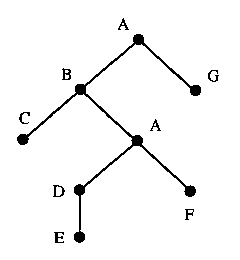
\includegraphics{ijbcf1.eps}
\end{center}
\caption{Labeled tree {\it T}.}
\label{fig2}
\end{figure}

\begin{sidewaysfigure}
\begin{center}
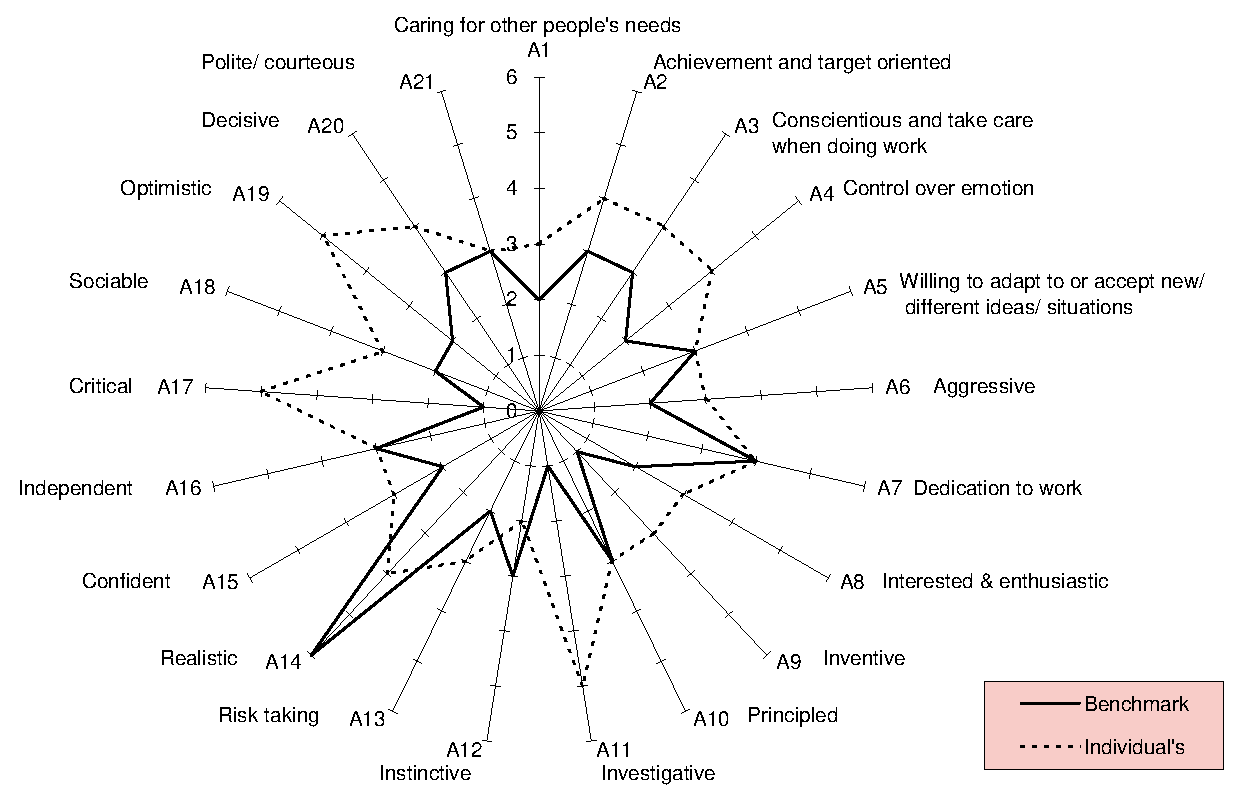
\includegraphics[width=7in]{ijbcf2.eps}
\end{center}
\caption{The bifurcating response curves of system
$\alpha=0.5, \beta=1.8; \delta=0.2, \gamma=0$: (a)
$\mu=-1.3$; and (b) $\mu=0.3$.}
\label{fig1}
\end{sidewaysfigure}

Figures are to be sequentially numbered with Arabic
numerals. The caption must be placed below the figure. For those
figures with multiple parts which appear on different pages, it is
best to place the full caption below the first part, and have
e.g.~``Fig.~1 ({\it continued})'' below the last part. Typeset in
9 pt Times Roman with baselineskip of 11 pt. Use double spacing
between a caption and the text that follows immediately.

Previously published material must be accompanied by written
permission from the author and publisher.

Very large figures and tables should be placed on a separate page
by themselves. Landscape tables and figures can be typeset with the following environments:
\begin{itemlist}
\item \verb|sidewaystable| and
\item \verb|sidewaysfigure|.
\end{itemlist}

\section{Tables}

\noindent Tables should be inserted in the text as close to the
point of reference as possible. Some space should be left above
and below the table. Tables should be numbered sequentially in the
text with Arabic numerals. Captions are to be centered above the
tables. Typeset tables and captions in 9 pt Times Roman with
baselineskip of 11 pt.

If tables need to extend over to a second page, the continuation
of the table should be preceded by a caption, e.g.~``Table~1 ({\it
continued})''.

\begin{table}[h]
\tbl{Number of tests for WFF triple NA = 5, or NA = 8.}
{\begin{tabular}{l c c c c c}\\[-2pt]
\toprule
{} &{} &3 &4 &8 &10\\[6pt]
\hline\\[-2pt]
{} &\phantom03 &1200 &2000 &\phantom02500 &\phantom03000\\[1pt]
{\ninebf NC} &\phantom05 &2000 &2200 &\phantom02700 &\phantom03400\\[2pt]
{} &\phantom08 &2500 &2700 &16000 &22000\\[2pt]
{} &10 &3000 &3400 &22000 &28000\\[1pt]
\botrule
\end{tabular}}
\end{table}

By using \verb|\tbl| command in table environment, long captions will be justified to the table width while the short or single line captions are centered.
\verb|\tbl{table caption}{tabullar environment}|.

For most tables, the horizontal rules are obtained by:

\begin{tabular}{ll}
{\bf toprule} & one rule at the top\\
{\bf colrule}& one rule separating column heads from data cells\\
{\bf botrule}& one bottom rule\\
{\bf Hline} & one thick rule at the top and bottom of the tables with multiple column heads\\
\end{tabular}

\

To avoid the rules sticking out at either end
of the table, add \verb|@{}| before the first and after the last descriptors, e.g.
{@{}llll@{}}. Please avoid vertical rules in tables.
But if you think the vertical rule is a must,
you can use the standard \LaTeX{} \verb|tabular| environment.

Headings which span for more than one column should be set using
\verb|\multicolumn{#1}{#2}{#3}| where \verb|#1| is the number of
columns to be spanned, \verb|#2| is the argument for the alignment
of the column head which may be either {c} --- for center
alignment; {l} --- for left alignment; or {r} --- for right
alignment, as desired by the users. Use {c} for column heads as
this is the WS style and \verb|#3| is the heading.

\section{Cross-references}
Use \verb|\label| and \verb|\ref| for cross-references to
equations, figures, tables, sections, subsections, etc., instead
of plain numbers. Every numbered part to which one wants to refer,
should be labeled with the instruction \verb|\label|.
For example:
\begin{verbatim}
\begin{equation}
\mu(n, t)=\frac{\sum\limits^\infty_{i=1}1 (d_i < t, N(d_i)=n)}
{\int\limits^t_{\sigma=0}1 (N(\sigma)=n)d\sigma}.\label{aba:eq1}
\end{equation}
\end{verbatim}
With the instruction \verb|\ref| one can refer to a numbered part
that has been labeled:
\begin{verbatim}
..., see also Eq. (\ref{aba:eq1})
\end{verbatim}

The \verb|\label| instruction should be typed
\begin{itemlist}
\item immediately after (or one line below), but not inside the argument of
a number-generating instruction such as \verb|\section| or \verb|\caption|, e.g.:
\verb|\caption{ ... caption ... }\label{aba:fig1}|.
\item roughly in the position where the number appears, in environments
such as an equation,
\item labels should be unique, e.g., equation 1 can be labeled as
\verb|\label{aba:eq1}|, where `{\tt aba}' is author's initial and
`{\tt eq1}' the equation number.
\end{itemlist}

\section{References}
References cited in the text should be placed within square
brackets and stated as [surname of author(s), year of
publication], e.g.. If the reference reads as part of
the sentence, the square brackets enclose only the year of
publication, e.g., ``According to Golub and Van Loan [1989], \ldots''

\nonumsection{Note Added} \noindent A note can be added before
Acknowledgments.

\nonumsection{Acknowledgments} \noindent This part should come
before References. Funding information may also be included here.

\nonumsection{Appendices} \noindent Appendices should be used only
when absolutely necessary. They should come immediately before
References.

\appendix{}
If there is more than one appendix, number them alphabetically.
\begin{equation}
\mu(n, t) = \frac{\displaystyle\sum^\infty_{i=1} 1(d_i < t, N(d_i) = n)}
{\displaystyle\int^t_{\sigma=0} 1(N(\sigma) = n)d\sigma}\,\,
.\label{that}
\end{equation}
Number displayed equations occurring in the appendix as (A.1),
(A.2), etc.


%\begin{thebibliography}{9}
\bibliography{sample}
%\end{thebibliography}

\end{document}
